\documentclass[11pt,letterpaper]{article}

\usepackage[font=footnotesize]{caption}
\usepackage{float}
\usepackage{epsf}
\usepackage{epsfig}
\usepackage{subfigure}
% \usepackage{subfig}
\usepackage{latexsym}
%\usepackage{algorithm}
%\usepackage[noend]{algorithmic}
% \usepackage{color}
\usepackage{color, colortbl}
\usepackage{wrapfig}
\usepackage{topcapt}
\usepackage{multirow}
\usepackage{tabularx}
\usepackage{hyperref}
\usepackage{xcolor}
\usepackage{mdwlist}
\usepackage{pdfpages} 
\usepackage{tabto}  
%\usepackage{color}
\newcommand{\lc}[1]{\textcolor{blue}{#1}}


\usepackage{amsmath, amsfonts, amssymb}
\usepackage[hmargin=1in,vmargin=1.2in]{geometry}
\usepackage{url}
\usepackage{multirow}
\usepackage[ruled,noline,linesnumbered]{algorithm2e}
\usepackage[bottom]{footmisc}
\usepackage{afterpage}
%\usepackage[caption=false]{caption}
\usepackage{eurosym}
\usepackage{enumitem}
% \usepackage{soul}
\usepackage{fancyhdr}
\usepackage{dashrule}
% \usepackage[stable]{footmisc}
% \usepackage{placeins}
% \setitemize{noitemsep,topsep=0pt,parsep=0pt,partopsep=0pt}
% \usepackage[utf8]{inputenc}
% \usepackage{gensymb}
\usepackage{rotating}
% \usepackage{tikz}
% \usepackage[firstpage]{draftwatermark} 

% \SetWatermarkText{DRAFT}
% \SetWatermarkScale{1}
% \SetWatermarkLightness{0}

% \interfootnotelinepenalty=80 
% \floatingpenalty=0\relax
\widowpenalty=1000
\clubpenalty=1000

\def\ls{{\texttt{LSTS\ }}}
\def\lse{{\texttt{LSTS}}}
\def\nas{{\texttt{NASA\ }}}
\def\nase{{\texttt{NASA}}}
\def\univ{{\texttt{UPorto\ }}}
\def\unive{{\texttt{UPorto}}}
\def\soc{{\texttt{SOCIB\ }}}
\def\soce{{\texttt{SOCIB}}}
\def\mit{{\texttt{MIT\ }}}
\def\mite{{\texttt{MIT}}}
\def\colo{{\texttt{Columbia\ }}}
\def\coloe{{\texttt{Columbia}}}
\def\ave{{\texttt{UAveiro\ }}}
\def\avee{{\texttt{UAveiro}}}
\def\inst{{\texttt{IH\ }}}
\def\inste{{\texttt{IH}}}
\def\sml{{SmallSat\ }}
\def\smle{{SmallSat}}

\def\org{{\texttt{RAND\ }}}
\def\orge{{\texttt{RAND}}}
\def\dec{{\texttt{UN Decade of the Oceans\ }}}
\def\dece{{\texttt{UN Decade of the Oceans}}}


\interfootnotelinepenalty=10000

\def\etal{{et al.\/}}
\def\eg{e.g., }
\def\ie{{i.e.,\ }}
\def\etc{{etc.\ }}
\def\situ{{in situ \/}}
\def\PN{{\emph{PN} }}

\definecolor{Gray}{gray}{0.6}


% \input{epsf}

% \newcommand{\rtime}[1]{\par\noindent\rlap{#1} \hspace*{2.15cm}}
% \newcommand{\iblank}{\par \noindent \hspace*{2.4cm} \hangindent 2.6cm}
% \newcommand{\m}[1]{\ensuremath{\mathbf{#1}}}
% \newcommand{\mc}[1]{\ensuremath{\mathcal{#1}}}
% \newcommand{\cn}{{\mathcal{CN}}}
% \newcommand{\ba}{\begin{align*}}
% \newcommand{\ea}{\end{align*}}

% \newcommand{\real}{{\mathbb{R}}}
% \newcommand{\integer}{{\mathbb{Z}}}
% \renewcommand{\natural}{{\mathbb{N}}}
% \newcommand{\argmin}{\operatorname{argmin}\displaylimits}
% \newcommand{\argmax}{\operatorname{argmax}\displaylimits}

% \newcommand{\relthresh}{{T_{\text{rel}}}}
% \newcommand{\absthresh}{{T_{\text{abs}}}}

% \newcommand{\nprof}{{N_{\text{prof}}}}
% \newcommand{\DM}{{DM}}
% \newcommand{\UM}{{UM}}
% \newcommand{\deltaMax}{{\partial_{\max}}}
% \newcommand{\IFD}{{IFD}}
% \newcommand{\IFU}{{IFU}}

% \newcommand{\mvdiff}{\mathbf{mvd}}
% \newcommand{\mvest}{\widehat{\mvdiff}}
% \newcommand{\prof}{p}

% \newtheorem{Prop}{Proposition}
% \newtheorem{Theorem}{Theorem}
% \newtheorem{Lemma}{Lemma}
% \newtheorem{Corrolary}{Corollary}

\def\be{\begin{equation}}
\def\ee{\end{equation}}

\newlength{\doublespacelength}
\setlength{\doublespacelength}{\baselineskip}
\addtolength{\doublespacelength}{0.5\baselineskip}
\newcommand{\doublespace}{\setlength{\baselineskip}{\doublespacelength}}

\newlength{\singlespacelength}
\setlength{\singlespacelength}{\baselineskip}
\newcommand{\singlespace}{\setlength{\baselineskip}{\singlespacelength}}


\newlength{\savedspacing}
\newcommand{\savespacing}{\setlength{\savedspacing}{\baselineskip}}
\newcommand{\restorespacing}{\setlength{\baselineskip}{\savedspacing}}

\setlength{\parskip}{0pt}
\setlength{\parsep}{0pt}
\setlength{\headsep}{0pt}
\setlength{\topskip}{0pt}
\setlength{\topmargin}{0pt}
\setlength{\topsep}{0pt}
\setlength{\partopsep}{0pt}
% \setlength{\parindent}{0pt}

\newtheorem{definition}{Definition}
\newcommand{\icomnt}[1]{{\color{red}{#1}}}
\newcommand{\kcomnt}[1]{{\color{blue}{#1}}}
\newcommand{\unit}[1]{\ensuremath{\mathrm{#1}}}                  %%%% to units and other roman math stuff

\newcounter{quotenumber}

\newenvironment{numquote}{%
    \begin{enumerate}%
     \setcounter{enumi}{\value{quotenumber}}%
     \color{darkgray}
    \item \begin{quote}%
}{%
    \end{quote}%
    \setcounter{quotenumber}{\value{enumi}}
    \end{enumerate}%
}%

\makeatletter
\def\myitem{%
   \@ifnextchar[ \@myitem{\@noitemargtrue\@myitem[\@itemlabel]}}
\def\@myitem[#1]{\item[#1]\mbox{}}
\makeatother



\newcommand\blankpage{%
    \null
    \thispagestyle{empty}%
    \addtocounter{page}{-1}%
    \newpage}

\setcounter{secnumdepth}{0} 

\let\oldthebibliography\thebibliography
\let\endoldthebibliography\endthebibliography
\renewenvironment{thebibliography}[1]{
  \begin{oldthebibliography}{#1}
    \setlength{\itemsep}{0em}
    \setlength{\parskip}{0em}
}
{
  \end{oldthebibliography}
}
% \linespread{0.98}
\parskip 0.1cm


\title{\Large{Integrating Modeling efforts in disaster resilience and planning:\\
    From observations to predictions}} 
\author{\normalsize{Kanna Rajan, Michelle Miro, Ajit
      Subramaniam~\footnote{Lamont Doherty Earth Observatory \&
        Columbia Climate School, \newline Columbia University,
        \url{https://lamont.columbia.edu/directory/ajit-subramaniam}}
    }\\
  \emph{\{Kanna.Rajan,mmiro\}@rand.org, ajit@ldeo.columbia.edu}\\
  \url{https://kanna.rajan.systems}}

\begin{document}

\maketitle{}
% \newpage

\subsection*{Executive Summary}

Extreme weather events are at a rise, with substantial increases not
only in intensity but also frequency. NOAA's National Centers for
Environmental Information, lists \$33 Million worth of property damage
from coastal events including Coastal Flood, Flash Flood, Storm
Surge/Tide, and Tropical storms in 227 events in 2022 alone, up from
201 events and \$25.5 Million worth of damage. Science and technology
have made rapid strides to predict such events and at a point where
modeling, systems, processes and strategies can be brought to bear to
mitigate human impact. Such tools can be used to stress-test the
preparedness of emergency responders and disaster management agencies,
while also providing strategic advice on asset allocation and
placement centrally focused on the importance of environmental
justice. 


\subsection*{Introduction}

The oceans covering more than 70\% of the Earth's surface are not only
a sink for Carbon, but also a major repository of the global capacity
to store heat from anthropogenic sources. The impact of rising sea
surface temperatures not only impacts marine life, but also human life
deep within terrestrial ecosystems with the increasing mass of heated
air transported from across the oceans over coastal boundaries, to
inland areas. The end result of such transport has led to floods, high
surf, hurricanes and tornados among other extreme events, not just in
coastal zones, but well inland. Even in urban areas, extreme events
have had a range of impacts with secondary effects from the
oceans. After effects of Hurricane Ida in Louisiana in 2021 led to an
excess of 3.91''/hour of rain in New York City, flooding basements in
Queens killing 11. \com{ajit: This is per hour - the point being that it is
  an extreme precipitation event with a large volume falling in a very
  short time.  The total rain across the region over the day was more
  like 6-8 inches}.

\subsection{Alternative Policy Need Section to replace two sections
  above}

Science and technology have made rapid strides in the prediction of
extreme weather events to a point where advanced monitoring and
modeling can be operationalized by emergency responders. By
integrating these advancements into planning tools, emergency managers
can stress-test the preparedness of emergency response and make
decisions on asset allocation and placement before disasters occur,
with the overall goal of minimizing impact on communities. Such
advancements can also incorporate the distributional effects of
disasters on communities, helping emergency response organizations and
others make decisions that reduce such inequities.


The integration of coastal riverine, land use and ocean dynamics
coupled with a logistical course of action (COA) will enable agencies
such as FEMA, Coast Guard and the Army Corps of Engineers to do ’what-
if-analyses’ to enhance preparedness. To do so, we need not just
models but hard and soft observations from a range of embedded and
on-the-ground sensors on mobile and static platforms (autonomous or
not) coupled with high resolution models with a predictive capability
which can be run effectively and quickly anytime.

\subsection*{Proposed Solution}

To limit loss of life and alleviate human suffering as a result of
such events, technology can and should play a prominent role. Higher
resolution ocean, atmospheric, estuarine and land use models can be
coupled to provide ways to enable 'what-if' analysis for policy makers
and other stakeholders. Increased model skill has resulted in better
predictions, but this is pre-medicated on having higher resolution
data at fine scales. Absent such high-resolution data, such models
cannot be effective in their forecasting precision. 

\begin{wrapfigure}{r}{0.45\textwidth}
  \centering
  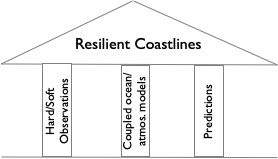
\includegraphics[scale=0.5]{fig/trioka.jpg}
  \caption{Predictive capacity go hand in hand with ocean/land use
    models derived from high resolution sensors from in-situ robotics.}
  \label{fig:tri}
\end{wrapfigure}

We believe the use of AI-driven networked mobile robotic platforms
carrying a range of payloads in space, aerial, surface, terrestrial
and underwater domains can provide the necessary capability for
precisely such data driven high-resolution prediction \com{ajit: I am not
  convinced that this particular configuration is necessary or even
  appropriate given that you need to deploy just before a storm}. They
can be targeted to be in the 'right place at the right time' as a
result of models being able to bound their own uncertainty. As a
result, the 'three poles' which enable such a responsive capacity
leading to coastal resilience include observations from hardware
robotic platforms, as well as Machine Learned methods mining troves of
remote sensing data all in high resolution, coupled ocean and
atmospheric models which can not only model the dynamic ocean and its
surface, but also interact with atmospheric phenomenon which provide
oceanographic forcing and finally the predictions for future
ocean/atmospheric state which can impact human habitation inland and
on shore (Fig. \ref{fig:tri}).

When these are combined with terrestrial land use, ecological and
hydrological models, a system-of-system then can provide stakeholders,
especially policymakers with a capability for 'what-if' scenario
generation at \textbf{block-by-block level} of urban environments,
which in turn can aid in the planning for extreme events for agencies
like FEMA especially in urban environments. 

Such tools can then be used in a number of ways, foremost being in
stress-testing the preparedness of emergency responders and disaster
management agencies, while also providing strategic advice on asset
allocation and placement. Another would be in using such ensemble
modeling for Monte-Carlo type repeat simulations to come up with the
most likely set of scenarios which could help in building planning
resilience.


\subsection*{Technical Details}

\begin{sidewaysfigure}[!]
  \centering
  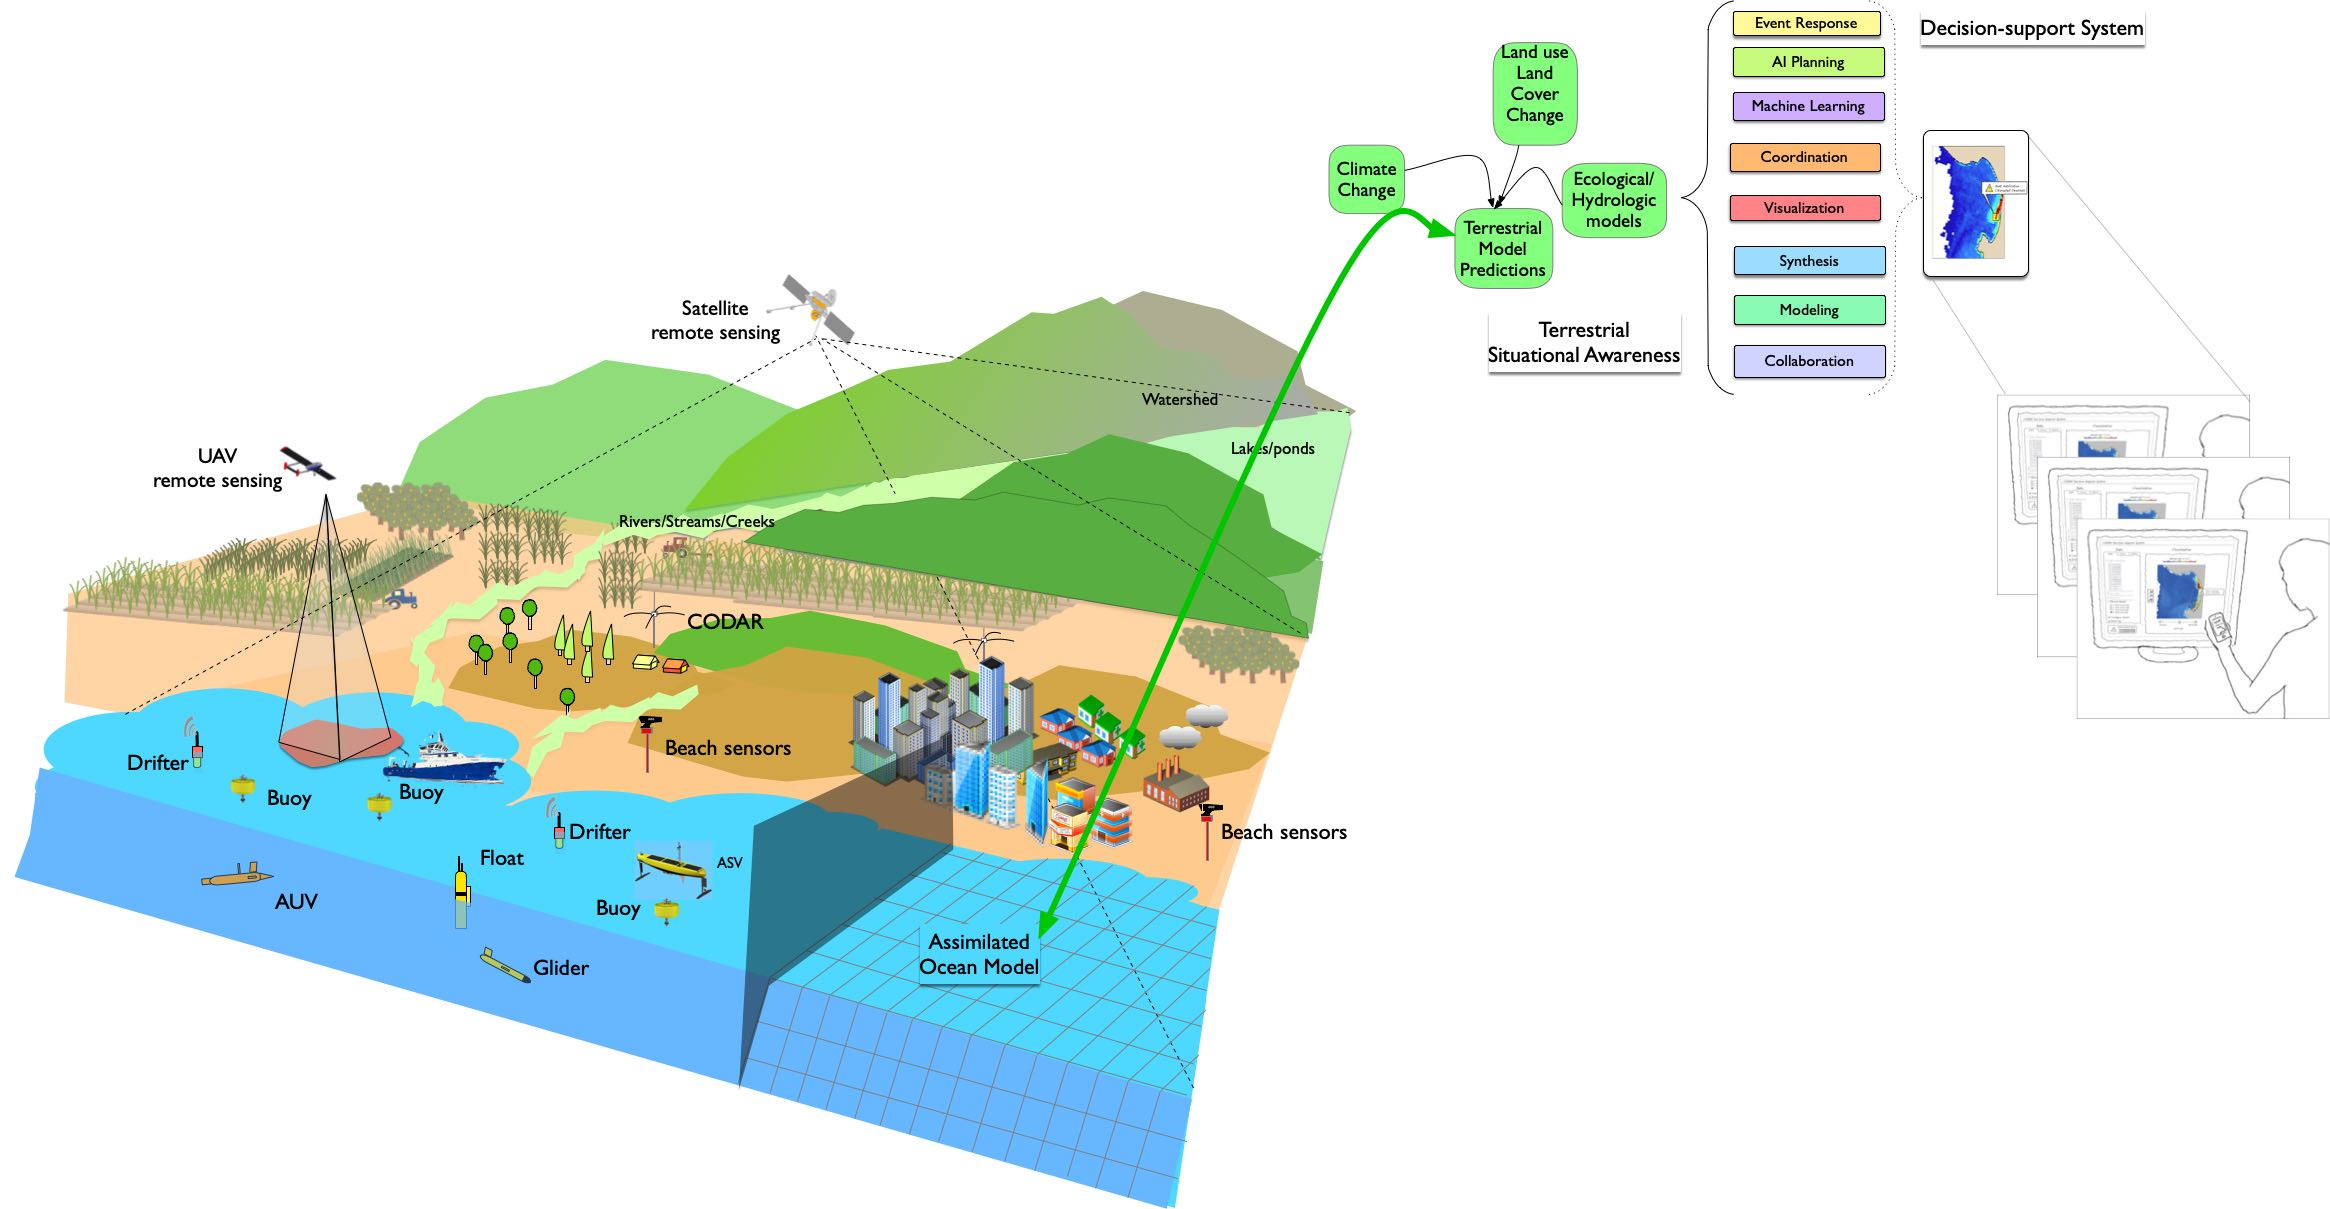
\includegraphics[scale=0.30]{fig/Coastal-connect.jpg}
  \caption{Networked space, aerial, surface, terrestrial and underwater
    platforms can gather high-resolution data in space and time to
    increase the predictive power of ocean driven extreme events.}
  \label{fig:coastal-res}
\end{sidewaysfigure}

\subsubsection*{Overview}

Extreme events are on the increase, impacting not only coastal
communities, but those deep within terrestrial domains, across the
world. Within the US, the typical Fall season has oceanic events
impacting coastal regions including flooding and extreme surf events
leading to large scale destruction of property and loss of lives. With
the increases in sea surface temperature and consequent energy stored
in the upper ocean, the atmospheric-ocean surface interaction has
become the driver for high intensity hurricanes well offshore and
tornadoes well inshore, as a means for captive energy transport. These
too have shown to lead to substantial and destructive impacts to human
lives and property. 

The oceans therefore are increasingly a key driver for such extreme
events. Our need to protect lives and property inland, including
coastal regions and urban centers at the block level, is increasingly
driven by what we need to know about the state of the oceans. This
form of interconnection is also related to how we are prepared for
natural emergencies which are endemic these days.

\subsubsection*{Sensor Network}


\begin{wrapfigure}{!r}{0.45\textwidth}
  \centering
  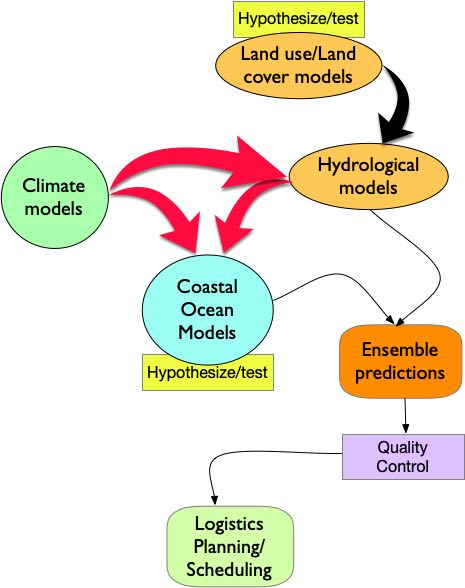
\includegraphics[scale=0.30]{fig/process.jpg}
  \caption{A range of predictive models will need to generate a QC-ed
    output, which can then be run into a logistics planning/scheduling
    engine during 'what-if' analyses.}
  \label{fig:process}
\end{wrapfigure}

We propose an \emph{integrative} effort to couple riverine/estuarine,
hydrologic and ocean models, driven by an ensemble of static and
mobile sensors on autonomous robotic platforms which sense-plan-act to
reduce modeling uncertainty, provide high resolution data and
consequent predictions, doing so with timeliness. An ensemble
prediction then combine these model outputs, to generate a final
prediction which must be quality-controlled (QC-ed) to drive a
logistics planning/scheduling tool. In so doing, a stakeholder can
seamlessly use the hypothesize/test function as a way to generate a
range of scenarios, which will automatically be incorporated into an
ocean or land use model. This would then trigger a novel prediction,
available for potential logistics planning (Fig. \ref{fig:process}).

To do so, we believe, networked mobile autonomous systems with an
AI-driven 'back end' software infrastructure can provide highly
effective ways to make not only 'what if' analyses for a range of
stakeholders for disaster management, but also provide targeted ways
in which the impact to various parts of the geography can be
estimated. Data is critical, especially for dynamically evolving
environmental conditions. To gather it, we need multiple ways and
multiple variables for measurement necessitating the need for a range
of platforms. Robotic platforms making in-situ measurements across the
aerial, surface and underwater domains (Fig. \ref{fig:coastal-res})
feed a range of calibrated sensor data to ocean models, which are
coupled with the local diurnal tidal cycle and estuarine predictions
can then make detailed predictions about the onset of offshore
climate's impact on the landmass. Predictions from shore then can be
propagated into a terrestrial/hydrological model to measure the impact
of high winds, tidal surges and hurricanes on inland communities.


\subsubsection*{System Modeling}

Typically land use, hydrological and ocean models are distinct,
derived and worked on in distinct communities with varied expertise.
We advocate an integrative approach to combine these methods in ways
that can provide decision-makers a valuable new tool which can be
portable across domains and demonstrate the power of integration.


\icomnt{Michelle, having some detail on how hydrologic and land use
  models (figures+text) work, plugged here would be useful. I'm
  basically guessing as to what their outputs might be (NetCDF?) and
  how they could be used.}

\begin{wrapfigure}{!r}{0.45\textwidth}
  \centering
  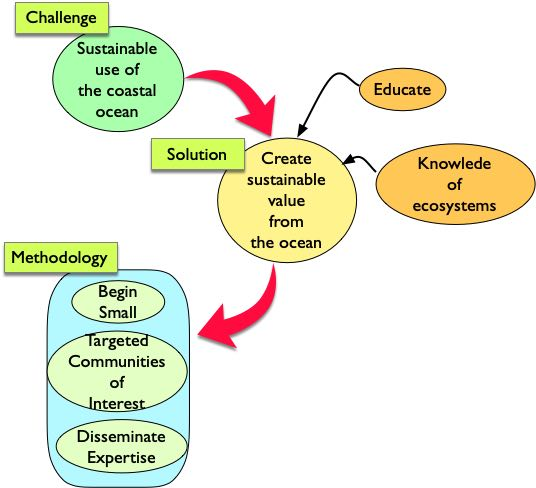
\includegraphics[scale=0.40]{fig/Ericeira-method.jpg}
  \caption{Using a mix of models integrated between coastal, terrestrial
    and land use methods could enhance sustainable ways of exploiting
    resources, both terrestrial and oceanic.}
  \label{fig:method}
\end{wrapfigure}


\subsubsection*{Integration}

Logistical considerations related to where (and when) emergency
management resources can then make targeted assessments of support
functions at precise locations and times. Legacy systems for disaster
preparedness could be interfaced with the ensemble
predictions. However, the power of Machine Learning methods could be
applied to ensure the right use of assets in ways that impact
assessments can be qualitatively measured to have the right assets at
the right place and time. 

This interconnected system-of-systems could used in a range of ways,
including in real-time disaster assessment, assessments of property
damage with aerial and space based remote sensing using before/after
imagery in targeted ways, as well as for multiple Monte-Carlo based
gaming assessments to hypothesize a range of diaster management
scenarios. These in turn could lead to Machine Learning based approaches
on high probability areas where logistical storage could be berthed in
order to have the maximum impact in terms of delivery and help to
victims of such natural events.

At a larger scale, climate models can be incrementally coupled into
such an ensemble of models to add to the longer term predictive power
(Fig. \ref{fig:coastal-res}) as a way to enhance estimation over
extreme cases. Not only will such an approach be critical for purposes
of resiliency, it will provide a range of stakeholder options on how
to make informed assessments on \emph{where} and \emph{when} to
provide support while enhancing sustainable use of resources both
coastal and terrestrial (Fig: \ref{fig:method}).



% \input{outcomes}


\section*{Concluding Remarks}

There is increasing need to have an integrative view of how coastal
and off-shore events tie into not only a predictive capability, but
also a tool-set to enable data/hypothesis driven informed policy which
in turn lead to concrete plans and actions for emergency responders in
shore and on land. The integration of coastal riverine, land use and
ocean dynamics coupled with a logistical course of action (COA) will
allow precisely such 'electronic table-top' driven exercises to
prepare agencies such as FEMA, Coast Guard and the Army Corps of
Engineers to do 'what-if-analyses' to ensure preparedness. To do so,
we need not just models but hard and soft observations from embedded
and in-situ sensors on mobile and static platforms (autonomous or not)
coupled with high resolution models with a predictive capability which
can be run effectively and quickly anytime. 

% \bibliographystyle{IEEEtran}
% {\footnotesize
% \bibliography{references}}

\end{document}